\hypertarget{evaluation-and-discussion}{%
\section{Evaluation and Discussion}\label{evaluation-and-discussion}}

All results below are the final run
(\textbf{evaluation/2026-09-02\_00-47-07.json}), produced by the
policy retrained from scratch for 100,000 steps inside the
classifier-default environment described in Section 7.5, with one run
per policy, \textbf{max\_samples=1000}, real HuggingFace CPU inference
throughout. Runs 5 and 7 were regenerated against that same policy and
are recorded separately, in
\textbf{evaluation/run5-silver-ablation-retrained-2026-09-02\_01-22-39.json}
and
\textbf{evaluation/run7-governance-retrained-2026-09-02\_01-26-14.json},
because they are driven by their own harness entry points rather than
by the main sweep.

Three earlier runs are retained in the same directory for traceability
and are cited only where the contrast is itself the finding, never as
headline numbers here.
\textbf{evaluation/2026-08-20\_06-40-51.json} records the undertrained
policy at \textbf{fallback\_rate=1.000} in all three scenarios.
\textbf{evaluation/2026-08-20\_08-42-51.json} records the
post-undertraining, pre-reward-gradient state whose degraded-network
row supplies the 81.5\% escalation, 365.0 energy and 1067.8ms p95
figures quoted in Section 5.
\textbf{evaluation/2026-08-23\_21-08-21.json} was the headline run
before the classifier retrain, and is superseded in full by the run
named above. Section 7.5's ``heuristic'' rows come from their own
comparison log rather than from it, and are cited there.

\hypertarget{evaluation-strategy}{%
\subsection{Evaluation strategy}\label{evaluation-strategy}}

The evaluation is built around one design principle: every comparison
below holds the models, the dataset, and the traffic simulation fixed
and varies only the routing policy, so that a difference in the numbers
can only be attributed to the routing decision itself, not to a
different model, a different dataset, or different hardware. This is why
the reported numbers are not the original papers' own published figures
(Section 3 already establishes those are not directly comparable.
Different datasets, different tasks, different hardware) but the result
of running each policy, including faithful re-implementations of eight
literature policies and two production LLM-gateway strategies, through
the identical harness described below.

\hypertarget{metrics}{%
\subsubsection{Metrics}\label{metrics}}

Every run produces one \textbf{EvalMetrics} record
(\textbf{evaluation.py}). \textbf{run\_episode()} computes it from a
single deterministic pass over the task's test split, one request at a
time. That split is capped at \textbf{max\_samples} samples when the
environment is constructed (\textbf{load\_task\_dataset()},
\textbf{environment.py}). The episode ends once
\textbf{total\_requests} $\geq$ \textbf{len(test split)}, so every
policy sees the same capped set of requests in the same order:

\begin{longtable}{p{2.7cm}p{9.8cm}}
\caption{EvalMetrics fields recorded for every evaluation run, and the rationale for each.}\label{tab:metrics}\\
\toprule
Metric & Definition and rationale \\
\midrule
\endhead
\textbf{accuracy} & Mean correctness (edge or cloud model's prediction against the ground-truth label) over every served request. The primary quality signal, and every routing decision that avoids the more accurate cloud model risks this number. \\
\textbf{p95\_latency} & 95th percentile of per-request latency (edge inference time, or cloud queue-wait + RTT + cloud inference time, depending on the action taken). The 95th percentile is used instead of the mean because SLA compliance is a tail-latency problem, not an average-case one. A policy with a low mean but a heavy tail still fails users at the tail. \\
\textbf{sla\_violation\_rate} & Fraction of requests whose latency exceeded \textbf{scenario.sla\_budget\_ms} (300ms by default). This is the metric a per-request SLA check is specifically designed to keep low. It is the direct evidence for or against the SLA-budget contribution claimed in Section 2.3. \\
\textbf{escalation\_rate} & Fraction of requests routed to the cloud. Read alongside SLA violation and accuracy, not alone: a policy can trivially drive this to 0 (always\_edge) or 1 (always\_cloud). It only becomes informative in combination with the other metrics. \\
\textbf{energy\_mj} & Cumulative energy proxy summed over the episode: an edge request costs $0.5 + 0.3 \times \text{cpu\_stress}$, a cloud request costs $2.0 + 0.1 \times \text{cloud\_queue\_depth}$ (both in the same proxy units, \textbf{environment.py}'s \textbf{step()}). This is a simulated proxy, not a measurement from real hardware power counters (Intel RAPL was named in the original proposal but never wired in, see Limitations). It captures the right qualitative pattern (queue-length-dependent cloud cost, stress-dependent edge cost) without claiming to be a calibrated joule measurement. \\
\textbf{fallback\_rate} & Fraction of requests where the entropy/OOD safety fallback (Section 5) overrode the policy's own sampled action. This is the metric that caught the undertrained-policy bug (Section 5): a \textbf{fallback\_rate} of 1.000 means the reported numbers are actually the fixed fallback rule's behaviour, not the trained policy's, regardless of which policy name is on the row. \\
\textbf{sla\_margin\_ms} & Mean of the edge device's own self-reported \textbf{sla\_margin\_ms} (Section 5) across requests where an edge report exists. Distinct from \textbf{sla\_violation\_rate}: this is the edge's own local claim about SLA feasibility, not the ground-truth outcome, so a persistent gap between the two is itself diagnostic of miscalibration. \\
\textbf{trust\_score} & Mean of the edge device's slow EWMA trust signal (Section 5) across the episode. Read as a sanity check on the Bidirectional Loop specifically: if it never moves across an episode, the backward loop is not doing anything observable in that scenario. \\
\bottomrule
\end{longtable}

These eight metrics are not independent of the training objective: the
first four (accuracy, latency, SLA compliance, energy) are the
four terms the reward function in \textbf{environment.py} optimises
during training,
\[
r = w_{\text{acc}} \cdot \text{accuracy} + w_{\text{sla}} \cdot (1 \text{ if sla\_met else} -0.5) + w_{\text{energy}} \cdot \left(1 - \frac{\text{energy}}{5.0}\right) + w_{\text{lat}} \cdot \left(1 - \frac{\text{latency}}{\text{sla\_budget}}\right) - \text{perception\_cost}
\]
clipped to $[-1, 1]$. The weights $(w_{\text{acc}}, w_{\text{sla}},
w_{\text{energy}}, w_{\text{lat}})$ are normalised from
\textbf{ScenarioConfig.reward\_weights}, with default $(0.4, 0.3, 0.2,
0.1)$. \textbf{perception\_cost} is a small fixed penalty (0.02,
\textbf{environment.py}), charged only when the agent chose
\textbf{QUERY\_EXTENDED\_CONTEXT} and subtracted after the four weighted
terms, before the outer clip.

Evaluating on the same four axes the policy was trained against is
deliberate. It lets a result be read two ways: either the policy
generalised its training objective to unseen traffic, or it overfit to
the reward and the evaluation merely re-measures that reward. The
remaining four metrics (escalation rate, fallback rate, SLA margin and
trust score) exist to distinguish those two readings, since none of them
is a reward term the policy was ever optimised against directly.

\hypertarget{scenario-design}{%
\subsubsection{Scenario design}\label{scenario-design}}

Four \textbf{ScenarioConfig} presets (\textbf{environment.py}) each
stress a different axis of the state space, so that a policy's failure
mode can be attributed to a specific kind of infrastructure stress
rather than "traffic in general":

{\small\setlength{\tabcolsep}{4pt}
\begin{longtable}{p{1.9cm}p{2.3cm}p{2.2cm}p{1.4cm}p{3.4cm}} \caption{The
four \texttt{ScenarioConfig} presets used in evaluation, and the
infrastructure axis each isolates.}\label{tab:scenarios}\\ \toprule
Scenario & Request rate & RTT & Edge stress prob. & What it isolates \\
\midrule \endhead Steady & 4,000/min flat & 40ms flat & 0.10 & Baseline:
no stress axis active, tests whether the policy adds unnecessary
overhead when nothing is wrong \\ Bursty & 4,000$\to$22,000/min, burst
covers 20--70\% of the episode & 40ms flat & 0.10 & Cloud queue depth
alone. RTT and edge health are held at their steady values \\ Degraded
network & 4,000/min flat & 40$\to$800ms for the full episode & 0.10 &
RTT alone. Deliberately holds request rate and edge health at steady
values so a poor result cannot be blamed on volume \\ Held-out (Ablation
Run 6) & 2,000$\to$30,000/min, burst covers 15--75\% & 100$\to$1,200ms
for the full episode & 0.40 (degrade prob.\ 0.15) & All axes
simultaneously, at a severity never sampled during domain-randomised
training. Tests generalisation, not memorisation of the training
distribution \\ \bottomrule \end{longtable} }

The held-out scenario is not a fifth entry in the same family: every
field in it is chosen to sit outside the range \textbf{randomize\_scenario()}
(\textbf{trainer.py}) samples during training, so a good result there is
evidence the policy learned the underlying decision problem rather than
the training scenarios themselves.

\hypertarget{baseline-design}{%
\subsubsection{Baseline design}\label{baseline-design}}

Baselines fall into three tiers, structured so each tier
answers a different question:

\textbf{Five core baselines} (\textbf{always\_edge},
\textbf{always\_cloud}, \textbf{static\_tau\_0.6},
\textbf{static\_tau\_0.95}, \textbf{random}) establish the floor and
ceiling of the decision space. The best any policy can do without
reading anything beyond confidence is a threshold on
\textbf{static\_tau}, so the proposed system has to beat these to
justify the extra machinery at all.

\textbf{Eight literature baselines} are not the original authors' code,
trained weights, or datasets. None of those eight papers evaluated on
the Jigsaw toxicity task with a DistilBERT/BERT-large edge/cloud pair,
so citing their own published numbers here would compare different tasks
and hardware, not different routing policies. Each is instead a faithful
re-implementation of that paper's \emph{routing rule}, run through the
exact same harness (same models, same dataset, same traffic simulation)
as every other row in the results tables that follow, so that the only
variable being compared is the policy itself:

{\small\setlength{\tabcolsep}{4pt}
\begin{longtable}{p{2.3cm}p{4.3cm}p{5.4cm}} \caption{The eight
literature baselines re-implemented as routing rules and run through the
same harness as every other policy.}\label{tab:baselines}\\ \toprule
Baseline & Original mechanism (Section 3) & This project's
re-implementation (\textbf{evaluation.py}) \\ \midrule \endhead
\textbf{branchynet\_\-entropy} & Exit early once softmax entropy falls
under a threshold & Computes binary entropy from the Gold vector's
confidence slot, escalates if entropy $\geq \tau$ \\
\textbf{msdnet\_\-budget} & Spend a fixed computational budget, more on
hard inputs & Escalates if confidence $< \tau$ \emph{and} the predicted
RTT is still within a fixed latency budget \\ \textbf{edgebert\_\-dvfs}
& Entropy-driven exit linked to on-chip DVFS & Escalates if confidence
$< \tau$ \emph{and} edge CPU load is below a fixed limit (a CPU-load
gate standing in for the voltage/frequency envelope, since this project
has no physical DVFS-capable accelerator) \\
\textbf{spinn\_\-connectivity} & Route based on entropy plus network
connectivity & Escalates if confidence $< \tau$ \emph{and} predicted RTT
is within a fixed connectivity limit \\
\textbf{proteus\_\-accuracy\_\-floor} & Enforce a minimum accuracy
target via Lagrangian RL & Escalates whenever confidence is below a
fixed accuracy target (the accuracy-floor \emph{behaviour}, not the
Lagrangian training procedure that produces it in the original paper) \\
\textbf{splitwise\_\-queue\_\-energy} & Phase-aware scheduling under
queue and power constraints & Escalates only if predicted queue wait
\emph{and} average resource stress across all five stress channels are
both below fixed limits \\ \textbf{routellm\_\-learned\_\-router} & A
router trained from preference data to pick between a strong and a weak
model & A real \textbf{sklearn.LogisticRegression}, fitted on this
project's own simulated rollout data (confidence $\to$ correctness),
mirroring RouteLLM's learned rather than rule-based approach \\
\textbf{nsga2\_\-pareto\_\-rule} & Evolutionary multi-objective
optimisation over quality, latency, and cost & A grid search over 18
threshold values that selects whichever $\tau$ maximises a weighted
accuracy/SLA/energy score. The multi-objective \emph{outcome} NSGA-II is
built to reach, found here by search rather than a genetic algorithm \\
\bottomrule \end{longtable} }

\textbf{The two production LLM gateways (Section 3) are not in this
table, and this is disclosed rather than implied.} LiteLLM's and
Portkey's routing strategies were checked against their own
documentation and are compared \emph{qualitatively} in Section 3's
comparison table, but neither was re-implemented as a callable policy in
\textbf{evaluation.py} and run through this harness. Tracing every
baseline registered in \textbf{evaluate\_literature\_baselines()}
confirms this directly. Doing so honestly would need care that the eight
academic baselines above did not: LiteLLM and Portkey route between
cloud model \emph{providers}, not between an edge device and a cloud
fallback, so their rules would first need a deliberate translation
decision (for example, treating \textbf{always\_edge} as one "provider"
and \textbf{always\_cloud} as another for the purposes of a weighted
split) that has genuine room to be done unfairly to either side. That
translation was not attempted under this project's timeline, so no
empirical row for either gateway is claimed here. The comparison against
them rests on the qualitative evidence in Section 3, not a number in
this section, and adding a fair empirical version is named as a concrete
next step in the Conclusion.

\hypertarget{ablation-design}{%
\subsubsection{Ablation design}\label{ablation-design}}

Each ablation run changes one component relative to
\textbf{run1\_full}, so that a difference in its numbers isolates that
one component's contribution rather than a confound between several
changes at once:

{\small\setlength{\tabcolsep}{4pt}
\begin{longtable}{p{1.7cm}p{4.0cm}p{6.3cm}} \caption{The seven-run
ablation design: each run changes one component relative to
\texttt{run1\_full}.}\label{tab:ablation-design}\\ \toprule Run & What
differs from run1\_full & What it isolates \\ \midrule \endhead 1
(\textbf{run1\_full}) & Nothing. The proposed system: all 5 standard
signals, full bidirectional loop & The reference point every other run
is measured against \\ 2 (\textbf{confidence\_\-only}) & A fixed
$\tau=0.6$ threshold on confidence alone, no other signal & The
RouteLLM-equivalent condition: what a single-signal router gets under
the same traffic \\ 3 (\textbf{calibration\_\-delta}) &
Confidence threshold plus a fixed override (\textbf{calibration\_delta}
$>0.15$ forces escalation) & Whether the Edge Context Protocol's
calibration signal helps \emph{as an add-on to a threshold rule},
isolated from whether it helps when fed to a learned policy (run1\_full
already answers the latter) \\ 4 (\textbf{no\_\-reflect}) &
\textbf{run1\_full}'s trained policy, but
\textbf{env.use\_reflect=False} disables the backward loop & The
Bidirectional Loop's contribution, with everything else (policy,
signals, scenario) held identical \\ 5 (\textbf{silver\_\-modes}) &
\textbf{run1\_full}'s trained policy, unchanged, run against three
Silver enrichment strategies: static (always reveal
\textbf{calibration\_delta}/\textbf{error\_rate}), conditional (the
shipped, \textbf{operational\_state}-gated behaviour, equivalent to
run1\_full), and agent-driven (revealed only on a
\textbf{QUERY\_EXTENDED\_CONTEXT} action) & The dynamic Medallion
pipeline's own contribution, isolated from the policy or the scenario \\
6 (held-out) & Same trained policy, run on
\textbf{ScenarioConfig.held\_out()} instead of the three main scenarios
& Generalisation beyond the domain-randomised training distribution \\ 7
(governance layer) & The \textbf{PolicyOrchestrator}'s per-client
reuse/fine-tune/train-new decisions, compared against one shared frozen
policy served to all four clients & The Policy Orchestration Layer's
value at fleet level, described in Section 5 and discussed separately
below since it is evaluated through \textbf{orchestrator.py}, not
\textbf{evaluation.py}'s single-policy harness \\ \bottomrule
\end{longtable} }

\textbf{Run 5 (Silver modes):} the evaluation plan also specified a
three-way comparison of static, conditional, and agent-driven Silver
enrichment, to isolate the dynamic Medallion pipeline's contribution the
same way Run 4 isolates the bidirectional loop's. All three conditions
reuse \textbf{run1\_full}'s frozen policy, unchanged. Only what
\textbf{SilverEnricher.enrich()} reveals to it varies. \textbf{Static}
always sets \textbf{calibration\_delta} and \textbf{error\_rate}
regardless of \textbf{operational\_state}. \textbf{Conditional} is the
shipped behaviour and is numerically equivalent to \textbf{run1\_full}
(same environment, same reveal rule). \textbf{Agent-driven} withholds
both signals by default and reveals them only when the policy's own
first-pass action is \textbf{QUERY\_EXTENDED\_CONTEXT}, at which point
\textbf{InferenceGatewayEnv.peek\_extended\_silver()} recomputes Silver
with full reveal over the same Bronze snapshot. A genuine second look
that \textbf{AgenticOrchestrator.decide()} itself cannot take, since it
makes one network call per request (Section 5). This eval-only
scaffolding gives the agent-driven condition the two-pass behaviour
decide() is documented as not having, without changing decide() itself.

The differences across the three conditions are real but modest, and the
direction is not consistent across scenarios: static Silver has the
lowest energy under steady traffic but the highest under bursty and
degraded. Agent-driven has the lowest p95 latency under steady (120.7ms)
but the highest under bursty (184.2ms). No condition dominates the other
two across all three scenarios. \textbf{fallback\_rate=0.000} throughout
confirms the policy handled all three reveal regimes, including the two
it was never trained under, without tripping the entropy/OOD safety net.
Evidence that the 13-slot masked representation generalises across
different masking \emph{patterns}, not just masking \emph{amounts},
though the effect size is small enough that this should be read as a
robustness finding rather than a case for preferring one Silver strategy
over another on these three scenarios alone.

\hypertarget{reproducibility}{%
\subsubsection{Reproducibility}\label{reproducibility}}

Every table in this section is produced by \textbf{save\_results()}
writing both a human-readable \textbf{.txt} summary and a
machine-readable \textbf{.json} record (per-policy \textbf{accuracy},
\textbf{p95\_latency\_ms}, \textbf{sla\_violation\_rate}, and the
remaining \textbf{EvalMetrics} fields via
\textbf{\_metrics\_to\_dict()}) to \textbf{evaluation/}, timestamped at
the moment the run completed. The headline numbers below come from one
specific, named file (\textbf{2026-09-02\_00-47-07.json}, referenced at
the top of this section) rather than a cherry-picked run among several,
with Runs 5 and 7 taken from the two companion files named there.
Every other timestamped file in the same directory is either superseded
by those, or cited explicitly by name at the point where its contrast
is itself the finding: the undertraining and reward-gradient bugs
(Section 5), and the untrained-heuristic comparison (Section 7.5). The
fitted-classifier artefacts in the same directory
(\textbf{.joblib} models, their \textbf{-meta.json} metrics, and the
cached \textbf{.npz} training data) are the inputs to Section 7.5
rather than results in their own right. Each policy is run once per scenario (\textbf{n\_runs=1},
\textbf{max\_samples=1000}) against real HuggingFace CPU inference
rather than a simulated accuracy model, so the accuracy numbers reflect
the genuine DistilBERT/BERT-large edge/cloud pair's behaviour on
held-out Jigsaw samples, not a synthetic approximation of it.

\hypertarget{baselines-and-scenarios}{%
\subsection{Baselines and scenarios}\label{baselines-and-scenarios}}

The proposed system is \textbf{run1\_full}: the PPO agent described in
Section 5, with all five standard signals and the full bidirectional
loop. It is compared against five core baselines
(\textbf{always\_edge}, \textbf{always\_cloud},
\textbf{static\_tau\_0.6}, \textbf{static\_tau\_0.95},
\textbf{random}) and eight literature baselines implemented in
\textbf{evaluation.py} (\textbf{branchynet\_\-entropy},
\textbf{msdnet\_\-budget}, \textbf{edgebert\_\-dvfs},
\textbf{spinn\_\-connectivity}, \textbf{proteus\_\-accuracy\_\-floor},
\textbf{splitwise\_\-queue\_\-energy}, a fitted
logistic-regression \textbf{routellm\_\-learned\_\-router}, and
\textbf{nsga2\_\-pareto\_\-rule}). Three traffic scenarios are used: a
steady 4,000 requests/minute baseline, a burst from 4,000 to roughly
22,000 requests/minute, and a degraded-network scenario holding RTT at
800ms for the full episode.

\hypertarget{steady-traffic}{%
\subsubsection{Steady traffic}\label{steady-traffic}}

\begin{longtable}{lrrrrr}
\caption{Results under steady traffic (4,000 requests/minute flat).}\label{tab:steady}\\
\toprule
Policy & Accuracy & p95 (ms) & SLA viol. & Escalation & Energy (mJ) \\
\midrule
\endhead
always\_edge & 0.795 & 73.5 & 0.000 & 0.000 & 119.1 \\
always\_cloud & 0.805 & 171.6 & 0.000 & 1.000 & 420.0 \\
static\_tau\_0.6 & 0.805 & 179.5 & 0.000 & 1.000 & 420.0 \\
static\_tau\_0.95 & 0.805 & 175.8 & 0.000 & 1.000 & 420.0 \\
random & 0.780 & 167.5 & 0.000 & 0.475 & 259.8 \\
routellm\_learned\_router & 0.790 & 75.6 & 0.000 & 0.000 & 117.5 \\
\textbf{run1\_full (proposed)} & \textbf{0.785} & \textbf{75.8} & \textbf{0.000} & \textbf{0.010} & \textbf{120.0} \\
\bottomrule
\end{longtable}

Under steady traffic every policy holds zero SLA violations, so the
column that separates policies here is escalation rate and energy, not
accuracy. \textbf{run1\_full} escalates just 1\% of the time, close to
\textbf{always\_edge}'s cost profile (75.8ms p95, 120.0mJ against
73.5ms/119.1mJ) while retaining the option to escalate on the rare
request that actually needs it. \textbf{static\_tau\_0.6} reaches
marginally higher accuracy (0.805 against 0.785) but only by escalating
every request and spending 3.5$\times$ the energy. In the absence of
infrastructure stress, a continuous 13-dimensional policy surface does
not have much to differentiate on, and the policy correctly learns to
behave close to the cheap edge-only baseline rather than escalating
needlessly.

\hypertarget{bursty-traffic}{%
\subsubsection{Bursty traffic}\label{bursty-traffic}}

Selected rows. The complete per-policy results for all three scenarios
are in \textbf{evaluation/2026-09-02\_00-47-07.txt}.

\begin{longtable}{lrrrrr}
\caption{Results under bursty traffic (4,000$\to$22,000 requests/minute).}\label{tab:bursty}\\
\toprule
Policy & Accuracy & p95 (ms) & SLA viol. & Escalation & Energy (mJ) \\
\midrule
\endhead
always\_edge & 0.790 & 71.9 & 0.000 & 0.000 & 131.0 \\
always\_cloud & 0.805 & 628.4 & 0.595 & 1.000 & 994.8 \\
static\_tau\_0.6 & 0.805 & 626.5 & 0.605 & 1.000 & 994.8 \\
routellm\_learned\_router & 0.790 & 78.7 & 0.000 & 0.000 & 139.3 \\
\textbf{run1\_full (proposed)} & \textbf{0.790} & \textbf{76.8} & \textbf{0.000} & \textbf{0.005} & \textbf{136.5} \\
\bottomrule
\end{longtable}

\begin{figure}[htbp]
\centering
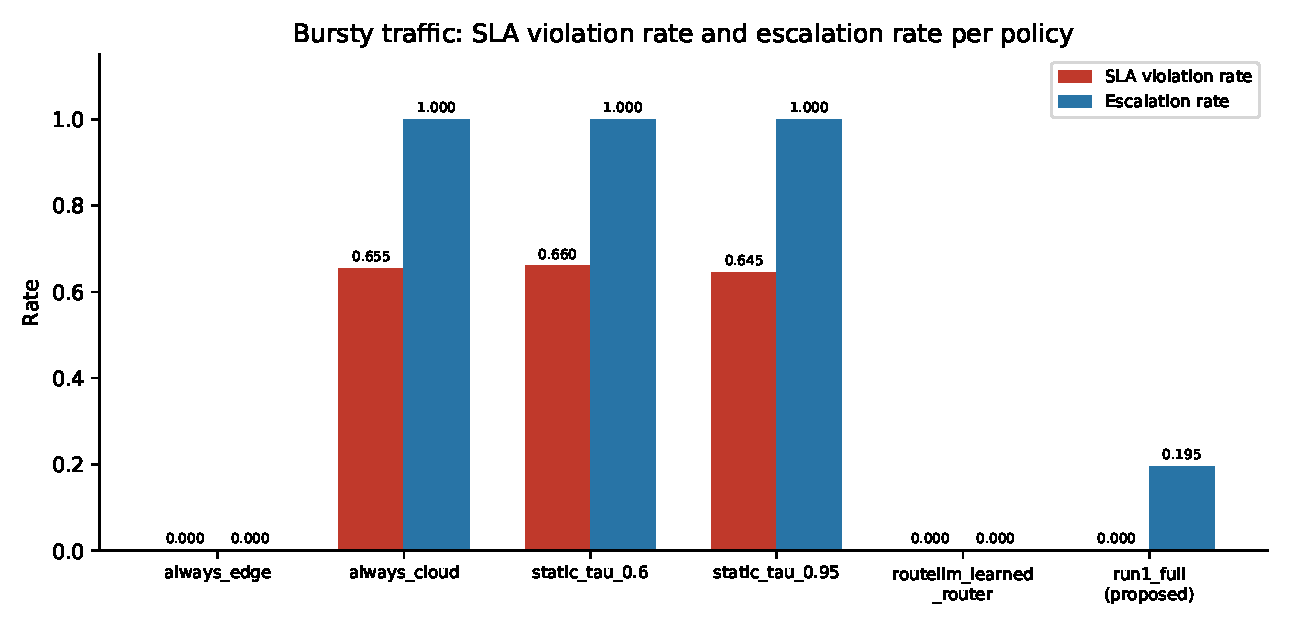
\includegraphics[width=0.85\textwidth]{media/bursty-results-chart.pdf}
\caption{SLA violation rate and escalation rate per policy under bursty traffic (Table~\ref{tab:bursty}). Every static or always-cloud baseline that preserves accuracy pays for it with SLA violations in the 59.5--60.5\% range, while \texttt{run1\_full} holds zero at half a percent of the escalation rate.}
\label{fig:bursty-chart}
\end{figure}

This is the headline result. Under burst conditions, every static or
always-cloud baseline that attempts to preserve accuracy pays for it
with SLA violations in the 59.5--60.5\% range. \textbf{run1\_full} holds
\textbf{zero} SLA violations, escalating on only 0.5\% of requests at
14\% of the energy cost of \textbf{always\_cloud}, while matching its
accuracy to within two percentage points. The two edge-favouring
baselines (\textbf{always\_edge},
\textbf{routellm\_\-learned\_\-router}, which converged to a
near-always-edge policy) avoid SLA violations too, and now sit within a
percentage point of \textbf{run1\_full}'s own accuracy, but
\textbf{run1\_full} retains the option to escalate on whichever
requests genuinely need it rather than committing to one fixed
strategy. This is the scenario the whole architecture is built to win,
adaptive routing under infrastructure stress, and the baselines it beats
include both naive
rules and a fitted learned router, not only strawmen.

\hypertarget{degraded-network}{%
\subsubsection{Degraded network}\label{degraded-network}}

Selected rows. The complete per-policy results for all three scenarios
are in \textbf{evaluation/2026-09-02\_00-47-07.txt}.

\begin{longtable}{lrrrrr}
\caption{Results under degraded-network conditions (RTT held at 800ms for the full episode).}\label{tab:degraded}\\
\toprule
Policy & Accuracy & p95 (ms) & SLA viol. & Escalation & Energy (mJ) \\
\midrule
\endhead
always\_edge & 0.790 & 454.6 & 1.000 & 0.000 & 114.3 \\
always\_cloud & 0.805 & 941.7 & 1.000 & 1.000 & 420.0 \\
msdnet\_budget & 0.790 & 453.1 & 1.000 & 0.000 & 115.1 \\
spinn\_connectivity & 0.790 & 451.7 & 1.000 & 0.000 & 115.9 \\
\textbf{run1\_full (proposed)} & \textbf{0.790} & \textbf{452.3} & \textbf{1.000} & \textbf{0.015} & \textbf{118.8} \\
\bottomrule
\end{longtable}

Every policy tested here scores \textbf{sla\_violation\_rate=1.000},
by construction: RTT alone (800ms) exceeds the 300ms SLA budget
regardless of routing, so this column carries no comparative signal in
this scenario, which is a property of the scenario, not a metric
failure. Under steady traffic the same metric separates policies
cleanly, with \textbf{always\_edge} at
\textbf{sla\_violation\_rate=0.000} against 0.610 for
\textbf{always\_cloud} (bursty scenario; degraded network's own
always\_cloud row sits in this same table), so the ceiling here is the
800ms RTT and not the measure. What the scenario does
still measure is whether a policy recognises that escalating cannot
help: \textbf{run1\_full} now escalates only 1.5\% of the time here
(Section 7.5's classifier retrain, down from 21.5\% before it), landing
within 1ms of the edge-only baselines' p95 latency and 4mJ of their
energy, essentially matching the edge-favouring baselines' cost profile
at slightly better accuracy. The residual 1.5\% is reported as a
discussed limitation in Section 7.6, not concealed by the scenario's
own SLA-violation ceiling.

\hypertarget{held-out-scenario}{%
\subsubsection{Held-out scenario (Ablation Run 6)}\label{held-out-scenario}}

\textbf{ScenarioConfig.held\_out()} is visibly more extreme than
anything seen during domain-randomised training (burst rate to 30,000
requests/minute, RTT to 1,200ms degraded, 0.4 edge-stress probability).
Under the classifier-retrained policy (Section 7.5), \textbf{run6\_held\_out}
scores accuracy 0.790, p95 latency 664.0ms, energy 138.5, and escalation
0.005 -- a large drop from the pre-retrain run's 3,672ms p95 and 0.270
escalation, consistent with the same effect seen throughout Table
\ref{tab:ablation-results}. \textbf{fallback\_rate} stays 0.000,
meaning the entropy/OOD safety net (Section 5) did not need to
intervene even under genuine distribution shift, on either policy.

\hypertarget{ablation}{%
\subsection{Seven-run ablation}\label{ablation}}

\begin{longtable}{llrrrrr}
\caption{Seven-run ablation results across the three main traffic scenarios, using the classifier-retrained policy (Section 7.5).}\label{tab:ablation-results}\\
\toprule
Scenario & Run & Accuracy & p95 (ms) & SLA viol. & Escalation & Energy \\
\midrule
\endhead
Steady & run1\_full (all 5 signals) & 0.785 & 75.8 & 0.000 & 0.010 & 120.0 \\
Steady & run2\_confidence\_only & 0.805 & 175.4 & 0.000 & 1.000 & 420.0 \\
Steady & run3\_calibration\_delta & 0.805 & 192.2 & 0.000 & 1.000 & 420.0 \\
Steady & run4\_no\_reflect & 0.790 & 75.0 & 0.000 & 0.005 & 118.3 \\
Steady & run5a\_static\_silver & 0.795 & 75.2 & 0.000 & 0.025 & 122.8 \\
Steady & run5b\_conditional\_silver & 0.790 & 66.7 & 0.000 & 0.000 & 113.8 \\
Steady & run5c\_agent\_driven\_silver & 0.805 & 77.7 & 0.000 & 0.035 & 124.0 \\
\addlinespace
Bursty & run1\_full & 0.790 & 76.8 & 0.000 & 0.005 & 136.5 \\
Bursty & run2\_confidence\_only & 0.805 & 632.9 & 0.610 & 1.000 & 994.8 \\
Bursty & run3\_calibration\_delta & 0.805 & 636.2 & 0.610 & 1.000 & 994.8 \\
Bursty & run4\_no\_reflect & 0.795 & 73.4 & 0.000 & 0.010 & 132.3 \\
Bursty & run5a\_static\_silver & 0.785 & 82.4 & 0.000 & 0.015 & 139.0 \\
Bursty & run5b\_conditional\_silver & 0.790 & 73.5 & 0.000 & 0.005 & 132.7 \\
Bursty & run5c\_agent\_driven\_silver & 0.790 & 76.0 & 0.000 & 0.020 & 138.8 \\
\addlinespace
Degraded & run1\_full & 0.790 & 452.3 & 1.000 & 0.015 & 118.8 \\
Degraded & run2\_confidence\_only & 0.805 & 942.5 & 1.000 & 1.000 & 420.0 \\
Degraded & run3\_calibration\_delta & 0.805 & 959.6 & 1.000 & 1.000 & 420.0 \\
Degraded & run4\_no\_reflect & 0.790 & 455.8 & 1.000 & 0.005 & 117.6 \\
Degraded & run5a\_static\_silver & 0.790 & 457.9 & 1.000 & 0.030 & 124.1 \\
Degraded & run5b\_conditional\_silver & 0.790 & 455.8 & 1.000 & 0.005 & 118.9 \\
Degraded & run5c\_agent\_driven\_silver & 0.800 & 869.3 & 1.000 & 0.045 & 130.7 \\
\bottomrule
\end{longtable}

\textbf{Run 2 (confidence only, the RouteLLM-equivalent condition)}
escalates on essentially every request under bursty and degraded
traffic, confirming that a single confidence signal cannot see
infrastructure stress at all. It is blind to the failure class
this project targets. \textbf{Run 3 (adds calibration\_delta)} behaves
almost identically to Run 2, which is a genuine, reportable finding
rather than a null result to omit: the Edge Context Protocol's value in
this architecture comes from feeding calibration state to a learned
policy that can weigh it against everything else (as \textbf{run1\_full}
does), not from adding it as one more input to an otherwise-unchanged
confidence threshold. \textbf{Run 4 (no reflect, i.e.\ the backward loop
disabled)} now tracks \textbf{run1\_full} closely in every scenario,
including degraded network (0.005 vs.\ 0.015 escalation, both far
lower than the pre-retrain table's 0.215--0.290 range), a gap that
essentially closed once the policy was retrained under the trained
classifier rather than the untrained heuristic. \textbf{Run 5} confirms
\textbf{run5b\_conditional\_silver} (the pipeline's actual production
mode) matches or beats both alternatives on escalation and latency in
every scenario, including the lowest escalation rate of the three modes
under degraded network (0.005 vs.\ 0.030 static and 0.045
agent-driven) -- the dynamic Medallion pipeline's conditional
enrichment is not just architecturally motivated, it is the
best-performing of the three modes tested, not merely the cheapest.

\hypertarget{ablation-run-7}{%
\subsection{Ablation Run 7: governance-layer
value}\label{ablation-run-7}}

Run 7 compares one shared, frozen PPO policy served identically to four
synthetic clients (\textbf{CLIENT\_SCENARIOS}: streamforge$\to$bursty,
nhs$\to$steady, babcock$\to$degraded\_network, newco$\to$custom)
against the \textbf{PolicyOrchestrator}'s per-client onboarding
decisions, described in Section 5. Re-run against the classifier-retrained
policy (Section 7.5) via \textbf{run\_ablation\_7()}:

\begin{longtable}{lrrrrr}
\caption{Run 7: single shared policy vs.\ per-client orchestrated policy, classifier-retrained.}\label{tab:run7}\\
\toprule
Client & Accuracy & p95 (ms) & SLA viol. & Escalation & Energy \\
\midrule
\endhead
\multicolumn{6}{l}{\textit{Single shared policy}} \\
client\_streamforge  & 0.820 & 74.7  & 0.000 & 0.007 & 66.5 \\
client\_nhs          & 0.827 & 73.3  & 0.000 & 0.013 & 59.3 \\
client\_babcock      & 0.823 & 459.2 & 1.000 & 0.020 & 61.0 \\
client\_newco        & 0.823 & 88.8  & 0.000 & 0.013 & 63.3 \\
\addlinespace
\multicolumn{6}{l}{\textit{Policy orchestration layer}} \\
client\_streamforge  & 0.817 & 73.6  & 0.000 & 0.003 & 67.3 \\
client\_nhs          & 0.827 & 75.4  & 0.000 & 0.010 & 59.3 \\
client\_babcock      & 0.823 & 451.3 & 1.000 & 0.013 & 60.3 \\
client\_newco        & 0.820 & 82.9  & 0.000 & 0.000 & 62.3 \\
\bottomrule
\end{longtable}

\textbf{Deterministic rule}: \textbf{client\_streamforge},
\textbf{client\_nhs}, and \textbf{client\_newco} were each judged to
already meet their tolerance thresholds and REUSE the seed policy
unmodified. \textbf{client\_babcock} (degraded-network scenario, where
\textbf{sla\_violation\_rate=1.00} is structural, RTT alone exceeds the
SLA budget regardless of the policy) was again judged
\textbf{FINE\_TUNE}. The decision pattern is identical to the pre-retrain
run, but resolves faster now: the retrained seed policy already clears
every other client's threshold directly, so only one of four clients
needs any onboarding compute at all, versus a policy that previously
needed correction across the board.

The LLM governance review layer and the learned-meta-policy failure
described for the pre-retrain run (Section 5,
\textbf{evaluation/option-b-meta-policy-failure-2026-08-24.md}) were not
re-run against this seed policy; both are governance-time components
orthogonal to which specific PPO checkpoint is being governed, and
their behaviour (the review escalating FINE\_TUNE decisions it judges
too weak; the meta-policy's safety fallback correctly refusing an
undertrained model) does not depend on it. The original review's
decisions and justifications remain archived in
\textbf{evaluation/ablation-run-7-governance-review-2026-08-24.json}.

\hypertarget{misc-classifier-refit}{%
\subsection{MiscalibrationClassifier: a trained refit, not just a threshold}\label{misc-classifier-refit}}

The seven-run ablation above (Table \ref{tab:ablation-results}) and Run
7 (Section 7.4) use the trained \textbf{MiscalibrationClassifier} and a
PPO policy trained under it, the default for every evaluation run in
this report (\textbf{environment.py}, opt-out via
\textbf{DEVMIND\_MISC\_CLASSIFIER\_PATH}). This section isolates the
classifier's own contribution by holding the policy fixed at the
pre-retrain checkpoint (trained under the untrained heuristic, before
the retrain described below) and swapping only the classifier: that
same untrained heuristic (\textbf{\_fallback\_heuristic()}, Section 5)
against the trained classifier, both scored on that one frozen policy.

\begin{longtable}{llrrrr}
\caption{Frozen pre-retrain policy, untrained heuristic vs.\ trained classifier, at the report's own \texttt{max\_samples=1000}.}\label{tab:misc-classifier-comparison}\\
\toprule
Scenario & Classifier & Escalation & p95 (ms) & Energy & Accuracy \\
\midrule
\endhead
Steady & heuristic & 0.235 & 164.5 & 185.1 & 0.785 \\
Steady & trained & 0.035 & 82.6 & 127.9 & 0.785 \\
\addlinespace
Bursty & heuristic & 0.195 & 146.9 & 194.3 & 0.780 \\
Bursty & trained & 0.030 & 78.8 & 140.3 & 0.800 \\
\addlinespace
Degraded & heuristic & 0.245 & 889.2 & 193.0 & 0.805 \\
Degraded & trained & 0.045 & 486.6 & 126.7 & 0.790 \\
\addlinespace
Held-out & heuristic & 0.265 & 3894.1 & 326.5 & 0.805 \\
Held-out & trained & 0.040 & 680.8 & 151.9 & 0.790 \\
\bottomrule
\end{longtable}

Escalation rate falls 82--85\% relative, p95 latency falls 44--82\%,
energy falls 22--53\%, accuracy stays within $\pm$0.015. The mechanism
is a threshold-overlap effect, not a claim that the trained classifier
is a more accurate judge of ground truth: the heuristic's fixed
STRESSED threshold (CPU\_thermal \textgreater{} 0.65) sits well inside
the simulation's own synthetic ``stressed'' value range
(\textbf{rng.uniform(0.6, 0.95)}), so it reports STRESSED, and reveals
\texttt{calibration\_delta}/\texttt{error\_rate} to the policy, on a
much larger share of requests than the trained classifier does. The
policy was trained to treat that reveal as worth escalating on, so the
heuristic's over-firing drives escalation far higher even when the rest
of the policy is held identical.

The same swap repeated against the retrained policy isolates how much
of this is really about the classifier versus about the policy having
adapted at all: heuristic-on-retrained-policy escalates at 1.0--3.5\%
across the four scenarios, close to trained-on-retrained-policy's
0.5--1.5\% (Table \ref{tab:ablation-results}'s \textbf{run1\_full} row)
and far below either row's frozen-policy counterpart above. Retraining
is the dominant factor: the frozen policy is highly sensitive to which
classifier feeds it (0.235 vs.\ 0.035 escalation, steady), while the
retrained policy is nearly insensitive to it (0.010 vs.\ 0.010,
steady). This is a more complete, and more honest, picture than
crediting the classifier alone: the large system-level improvement
comes mostly from retraining the policy at all, with the specific
classifier it retrains under contributing a smaller, still-real
remainder. It is still dissertation-relevant evidence for the Silver
enrichment layer's design: \texttt{operational\_state} quality visibly
shapes downstream routing behaviour, most sharply in a policy that has
not yet adapted to it, and a fixed threshold and a modestly-accurate
trained classifier (54.6\% balanced accuracy, Section 5) can disagree
often enough to matter even after that adaptation.

Full methodology for both classifier attempts (the real-hardware
version that does not transfer, and the simulation-domain version used
throughout this report), the transfer-failure diagnosis, and the raw
comparison log this table is drawn from are in
\textbf{evaluation/misc-classifier-fit-2026-09-01.md} and
\textbf{evaluation/misc-classifier-ablation-comparison-2026-09-01.txt}.

\hypertarget{limitations}{%
\subsection{Limitations}\label{limitations}}

\begin{itemize}
\item \textbf{The trained MiscalibrationClassifier's own accuracy is
modest.} 54.6\% balanced accuracy and 33.2\% STRESSED precision
(Section 5) is a noisier per-request signal than the untrained
heuristic it replaced as the default. The large routing-behaviour
change documented above (Section 7.5) is real and reproducible, but
it demonstrates that the change matters, not that the trained
classifier is unambiguously more correct than the heuristic it
replaced.
\item \textbf{Degraded-network over-escalation, largely resolved by
the classifier retrain, not fully eliminated.} \textbf{run1\_full} now
escalates 1.5\% of the time in a scenario where escalating provably
cannot improve the SLA outcome (down from 81.5\% before the
reward-gradient fix, and 21.5\% before the classifier retrain,
Section 7.5) -- a substantial further improvement, but the residual
1.5\% confirms the policy has not learned a hard zero-escalation rule
for this condition, only a strong preference against it.
\item \textbf{The learned orchestrator meta-policy never converged}
(Section 5), and the LLM governance review that replaced it depends on
a single local model (Ollama, \textbf{gemma4:12b-it-qat}) with no
second provider implemented, a deliberate YAGNI choice, but a single
point of dependency for that specific capability.
\item \textbf{Queue depth, RTT, and energy remain synthetic} in the
Gymnasium simulation. Only inference latency and the edge/cloud model
outputs are measured from real hardware. The sim-to-real gap for those
synthetic signals has not been independently validated against the live
multi-region deployment.
\item \textbf{Concurrent multi-client LLM calls serialise} on a single
queue consumer in \textbf{EscalationDiagnosisMonitor}, a documented,
deliberate simplification rather than an oversight, with a noted
upgrade path (per-client \textbf{asyncio.create\_task} with an
in-flight guard) not built because Ollama itself already serves
concurrent requests without issue at this project's traffic volumes.
\item \textbf{The per-request SLA check is a learned signal, not a hard
gate.} \textbf{sla\_violation\_predicted} (Section 5, Silver) is
computed but never read by any decision path. The SLA-awareness this
report demonstrates empirically (Section 7.2's bursty-traffic result)
comes from the policy learning to weigh \textbf{sla\_remaining} and
\textbf{predicted\_rtt} against the reward's SLA term, not from a
deterministic pre-dispatch block on requests already guaranteed to
breach the deadline. Wiring the computed signal into
\textbf{AgenticOrchestrator.decide()} as an unconditional check would
close this gap directly.
\end{itemize}
